\documentclass{article}
\usepackage[left=0.85in, right=0.85in, top=0.5in, bottom=0.95in]{geometry}
\usepackage[T1]{fontenc}
\usepackage[utf8]{inputenc}
\usepackage[italian]{babel}
\usepackage{graphicx}
\usepackage{wrapfig2}
\usepackage{amsmath}
\usepackage{amssymb}
\usepackage{cases}
\usepackage{subcaption}
\usepackage{hyperref}
\hypersetup{
	colorlinks=true,
	linkcolor=blue,    
	urlcolor=blue,
	pdfpagemode=FullScreen,
}
\urlstyle{same}
\usepackage{changepage}
\usepackage{lastpage, epstopdf}
\usepackage{fancyhdr}
\usepackage{tcolorbox}
\usepackage{background}
\usepackage{color}


%=======HEADER & FOOTER=======%
\def\lesson{Lesson Title}
%\def\outcome{\textbf{Learning Outcomes:} Outcomes go here. }

%\pagestyle{fancy}
%\fancyhf{}
%\renewcommand{\headrulewidth}{0pt}
%\renewcommand{\footrulewidth}{1.4pt}
%\lfoot{My Name $\diamond$ \the\year}
%\cfoot{Page \thepage/\pageref{LastPage}}
%\rfoot{\lesson}

%=======CORNELL STYLE FORMAT=======%
\SetBgScale{1}
\SetBgAngle{0}
\SetBgColor{black}
\SetBgContents{\rule{1pt}{0.899\paperheight}}
\SetBgHshift{-1.6in}
\SetBgVshift{-0.1in}

%=======CUSTOM BOXES=======%

\parindent 0ex

%=======BODY=======%
\begin{document}
%	\setcounterpageref{secnumdepth}{0}
	\section*{MECCANICA DEI SOLIDI: PARTE 3} %Date: \hrulefill}
%	\begin{tcolorbox}{\outcome}\end{tcolorbox}
	
	\begin{adjustwidth}{2in}{} 
		
	{\Large \textbf{Centro di Spostamento}} \mbox{} \newline
Ciò che interessa in questo senso è mettere a punto un sistema che permetta di studiare il moto della struttura senza ogni volta dover affrontare calcoli. \newline
	
Un generico campo di spostamento (CDS) è dato da:
\[
\vec{s_P} = \vec{s_0} + \vec{\Phi} \times (P-O)
\]		
Ovvero, nel riferimento assoluto nel piano lo spostamento è individuabile tramite un vettore traslazione parallelo al piano e un vettore rotazione ortogonale al piano.	\newline

NB: Punto fermo $\rightarrow$ punto a spostamento nullo, centro di istantanea rotazione. Punto per il quale l'atto di moto è descrivibile mediante una sola rotazione. \newline

La definizione di centro di spostamento è:: 
\[
\vec{s_P} \ne 0 \Rightarrow ~ \exists! ~ C :
\]
È ovvero caratterizzato da spostamento nullo. 
\begin{enumerate} 
\item $\vec{s_C} = 0$
\item $\vec{s_P} = \vec{\Phi} \times (C-O)$
\item La retta passante per C ed O è $\perp \vec{s_0}$, con O $\in$ al generico piano mobile.
\end{enumerate}
Dimostrazione (1,2):
\[
\begin{cases}
	\vec{s_P} = \vec{s_C} + \vec{\Phi} \times (P-O) \\
	\vec{s_C} = 0
\end{cases} \Rightarrow \vec{s_P} = \vec{\Phi} \times (P-O)
\]
Dimostrazione (1,3):

Si cerca un punto C tale che: $\vec{s_C} = 0$. 

Lo spostamento del punto C rispetto ad un polo O è dato da: $\vec{s_C} = \vec{s_0} + \vec{\Phi} \times (C-O)$.

Moltiplico entrambi i membri per il vettore rotazione:
\[
\vec{\Phi} \times \vec{s_C} =\vec{\Phi} \times \left[ \vec{s_0} + \vec{\Phi} \times (C-O)\right] 
\]
E dunque:
\[
0 =\vec{\Phi} \times \left[ \vec{s_0} + \vec{\Phi} \times (C-O)\right] 
\]	
\[
\vec{\Phi} \times \vec{s_0} + \vec{\Phi} \times \vec{\Phi} \times (C-O) = 0
\]		
Ricordando la proprietà dei vettori per cui: 
\[
\vec{a} \times \vec{b} \times \vec{c} = -(\vec{a} \cdot \vec{b}) \cdot \vec{c} + (\vec{a} \cdot \vec{c}) \cdot \vec{b}
\]		
Allora: 
\[
\vec{\Phi} \times \vec{s_0} - (\vec{\Phi} \cdot \vec{\Phi}) \cdot (C-O) = 0
\]		
\[
\vec{\Phi} \times \vec{s_0} = \vert\vec{\Phi}\vert^2  \cdot (C-O) 
\]	
\[
(C-O) = \frac{\vec{\Phi} \times \vec{s_0}}{\vert\vec{\Phi}\vert^2} \Rightarrow (C-O) \perp \vec{s_0}, (\vec{\Phi} )
\]
Poiché (C-O) si configura essere il risultato di un prodotto vettoriale, sarà sicuramente perpendicolare ad $\vec{s_0}$.

Ed indica che C è punto proprio. \newline

Osservazione: cosa accade se il corpo si muove per pura traslazione? Come faccio a esprimere la rotazione di un corpo attorno al suo CdS? \newline

Se il moto è di traslazione pura $\vec{\Phi} = 0$ allora, valendo ancora 1,2,3:
\[
(C-O) = \lim\limits_{\vec{\Phi} \rightarrow 0} \frac{\vec{\Phi} \times \vec{s_0}}{\vert\vec{\Phi}\vert^2} \rightarrow +\infty
 ~~~~ \blacksquare\]
La distanza (C-O) è infinita stando ad indicare che C sta all'infinito, ovvero è un punto improprio sempre per definizione in direzione ortogonale ad $\vec{s_0}$. \newline

\textbf{TEOREMA} \newline
Per un corpo/piano.

\[
\text{Se} ~ \exists ~ C_1,C_2 ~ \text{con} ~ C_1 \ne C_2 : \begin{cases}
\vec{s_{C_1}} = 0 \\
\vec{s_{C_2}} = 0
\end{cases} \Rightarrow \vec{s_P} = 0 ~ \forall ~ P 
\]
Tutti i punti P appartenenti al quel piano sono fermi.
Come dev'essere un punto per essere un candidato CdS? Dev'essere fermo. 
Cioè, se si hanno due punti candidati ad essere centro di spostamento, allora lo spostamento del campo è quello banale, quello nullo, non esiste il CdS perché se esiste è unico. \newline

NB: Per definire un punto nello spazio ho sempre bisogno di due informazioni, se il punto è proprio allora avrò le coordinate (x,y) o la direzione e la posizione del vettore, se il punto è improprio saprò che sarà all'infinito e dovrò sapere la direzione. \newline

Dimostrazione: 

\[
\begin{array}{c}
	\text{Spostamento di P generico rispetto a $C_1$} \\
	\vec{s_P} = \vec{s_{C_1}} + \vec{\Phi}\times (P-C_1)
\end{array}  \hspace{2cm}
\begin{array}{c}
		\text{Spostamento di $C_2$ rispetto a $C_1$} \\
 \vec{s_{C_2}} = \vec{s_{C_1}} + \vec{\Phi} \times (C_2-C_1)
\end{array}
\]
Ma per ipotesi $ \vec{s_{C_1}} = 0 = \vec{s_{C_2}}$, allora:

\[
\begin{cases}
	0 = \vec{s_{C_2}} = \vec{\Phi} \times (C_2-C_1) \\
	\vec{s_P} = \vec{\Phi} \times (P-C_1)
	\end{cases} \Rightarrow \vec{s_P} = 0  
\] 
$C_1 \ne C_2 \ne 0$: sono punti distinti $\blacksquare$ \newline 

{\Large \textbf{Centro di Spostamento Relativo}} \mbox{} \newline
Anche per un campo di spostamento relativo posso definire un CdS.
\begin{figure}[H]
	\centering
	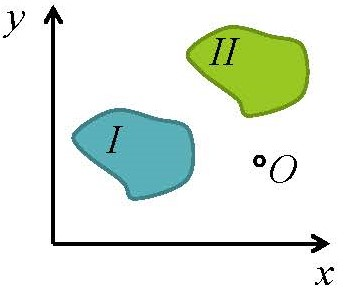
\includegraphics[width=0.2\linewidth]{immagini/1.PARTE3_Pagina_06}
\end{figure}

Dati nel piano mobile due corpi 1 e 2 in movimento relativo e un polo O, si può scrivere:
\[
\begin{cases}
\vec{s_P}' = \vec{s_0}' + \vec{\Phi}' \times (P-O) \\
\vec{s_P}'' = \vec{s_0}'' + \vec{\Phi}'' \times (P-O) \\
\vec{s_P}^{'', '} = \vec{s_0}^{'', '}  + \vec{\Phi}^{'', '}  \times (P-O) 
\end{cases}
\]

Analogamente, la definizione di centro di spostamento relativo è: 
\[
\vec{s_P}^{'', '} \ne 0 \Rightarrow ~ \exists! ~ C_{12} :
\]
Si potrà perciò avere anche spostamento assoluto non nullo, ma quello relativo dovrà essere nullo. 
\begin{enumerate} 
	\item $\vec{s_{C_{12}}}^{'','} = 0$
	\item $\vec{s_P}^{'','} = \vec{\Phi}^{'','} \times (P-C_{12})$
	\item La retta passante per C ed O è $\perp \vec{s_0} \Rightarrow (C_{12}-O) = \frac{\vec{\Phi}^{'','} \times \vec{s_0}^{'','}}{\vert\vec{\Phi}^{'','}\vert^2} $
\end{enumerate}
Inoltre: 
\[
C_{12} = C_{21}
\]
 \[
 \begin{cases}
\vec{s_0}^{'','} = -\vec{s_0}^{',''} \\
\vec{\Phi}^{'','} = - \vec{\Phi}^{',''}
 \end{cases} \Rightarrow (C_{21}-O) = \frac{\vec{\Phi}^{',''} \times \vec{s_0}^{',''}}{\vert\vec{\Phi}^{',''}\vert^2} = - \frac{\vec{\Phi}^{'','} \times \vec{s_0}^{'','}}{\vert\vec{\Phi}^{'','}\vert^2} = \frac{\vec{\Phi}^{'','} \times \vec{s_0}^{'','}}{\vert\vec{\Phi}^{'','}\vert^2} = (C_{12}-O) 
 \] \newline

\textbf{PRIMO TEOREMA DELL'ALLINEAMENTO} \newline
Dato $C_1$ il centro di spostamento del corpo 1 e $C_2$ il centro di spostamento del corpo 2 e $C_{12}$ il centro di spostamento relativo, affinché il moto NON sia banale, la condizione necessaria e sufficiente è che i tre Centri di Spostamento siano allineati.

Dimostrazione \textbf{HOMEWORK}

Hint: Se i CdS giacciono sulla stessa retta allora sono allineati e c'è spostamento, se non sono allineati non c'è spostamento e non esiste alcun CdS.

(1)\textbf{Corollario: unicità del centro di spostamento} \newline
Se esistono due punti $P_1, P_2$ tali che $\vec{s_{P_1}} = \vec{s_{P_2}} = 0$ allora il corpo è fermo poiché non può esistere più di un centro di spostamento, difatti, se esso esiste, è unico. \newline

(2)\textbf{Corollario: corpo fermo} \newline
Se si hanno due corpi mobili e i punti $C_1, C_2, C_{12}$ sono possibili candidati ad essere centri di spostamento e se: 
\[
C_1 = C_{12} \ne C_2
\]
Allora il corpo 2 è fermo.

Il corpo I ruota intorno a $C_1$; il corpo II ruota intorno a $C_2$; $C_{12}$ si può vedere come centro relativo del moto che compie I intorno a II, punto che si vedrà fermo se ci si mettesse a cavallo del corpo II, ma che, se combacia con quello assoluto, si vede fermo per definizione. 

Dimostrazione:
\[
\begin{cases}
\vec{s_{C_1}}' = 0 \\
\vec{s_{C_2}}'' = 0 \\
\vec{s_{C_{12}}}^{'','} = 0
\end{cases} \Rightarrow \begin{cases}
\underbrace{\vec{s_{C_{12}}}'' = \vec{s_{C_{12}}}' + \vec{s_{C_{12}}}^{'','}}_\text{Per definizione di spostamento relativo} = \vec{s_{C_{12}}}^{'','} \\
C_1 = C_2
\end{cases} \Rightarrow \vec{s_{C_{12}}}'' = \vec{s_{C_{12}}}' = \vec{s_{C_1}}' = 0
\]
Ho un secondo candidato ad essere centro di spostamento assoluto per il corpo II, il che significa che il corpo è fermo. $ ~~~~ \blacksquare $ \newline

(3)\textbf{Corollario: corpo fermo} \newline
Se si hanno due corpi mobili e i punti $C_1, C_2, C_{12}$ sono possibili candidati ad essere centri di spostamento e se: 
\[
C_1 = C_2 \ne C_{12} 
\]
Allora non si ha spostamento relativo tra i corpi.
\[
\vec{s_P}^{'','} = 0
\]
\[
\begin{cases}
	\vec{s_{C_1}}' = 0 \\
	\vec{s_{C_2}}'' = 0 \\
	\vec{s_{C_{12}}}^{'','} = 0
\end{cases} \Rightarrow \begin{cases}
	\vec{s_{C_{2}}}^{'','} = \vec{s_{C_{2}}}' + \vec{s_{C_{2}}}^{''} = \vec{s_{C_{2}}}^{'} \\
	C_1 = C_2
\end{cases} \Rightarrow \vec{s_{C_{2}}}^{'','} = \vec{s_{C_{2}}}' = \vec{s_{C_1}}' = 0
\]
$C_2$ è centro del moto relativo. $ ~~~~ \blacksquare $ \newline

\textbf{SECONDO TEOREMA DELL'ALLINEAMENTO} \newline
Si considerino 3 corpo di una struttura labile, se esistono i punti $C_{12}, C_{13}, C_{23}$ centri di spostamento relativo, allora essi sono allineati. \newline 




\newpage
{\Large \textbf{Centro di Spostamento e Vincoli}} \mbox{} \newline

Posso trovare informazioni sui CdS senza dover analizzare gli spostamenti dei singoli corpi? Con i vincoli?

Un vincolo consiste in una restrizione cinematica del corpo.

Il centro di spostamento è il punto di rappresentazione della cinematica del corpo.

Esiste dunque una relazione tra i vincoli e i centro di spostamento che permette di studiare la labilità di una struttura e tracciarne le catena cinematica. 
\begin{itemize}
\item \textbf{Cerniera} $\vec{s_A} = 0 \Rightarrow ~ \text{se} ~ \exists ~ C \Rightarrow C \equiv A$
\begin{figure}[H]
	\centering
	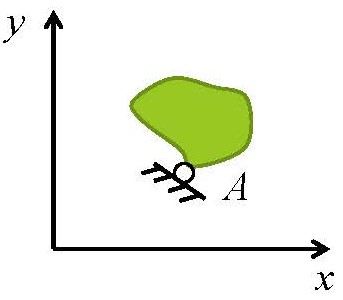
\includegraphics[width=0.15\linewidth]{immagini/1.PARTE3_Pagina_10 (2)}
\end{figure}
La cerniera impedisce lo spostamento del punto a cui è applicata, ricordi che aveva MC=2? La cerniera fornisce due informazioni sulla posizione del CdS, due informazioni in un piano definiscono un punto. 

\item \textbf{Pendolo} $\vec{s_A} \cdot \vec{e} = 0 \Rightarrow ~ \text{se} ~ \exists ~ C \Rightarrow C ~ \in e$
\begin{figure}[H]
	\centering
	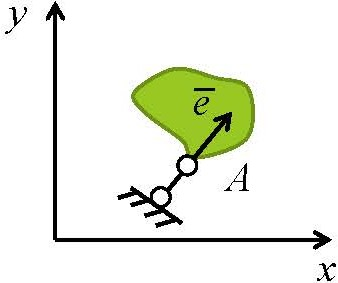
\includegraphics[width=0.15\linewidth]{immagini/1.PARTE3_Pagina_10}
\end{figure}
So che $\vec{s}_A \perp \vec{e}$ Dove si troverà C? Lungo la direzione perpendicolare ad $\vec{s}_A$ e dunque apparterrà ad $\vec{e}$. 

MC=1, il pendolo fornisce una sola informazioni sulla localizzazione del Csd: la sola direzione. 
\item \textbf{Doppio Pendolo} $\begin{cases}
	\vec{s_A} \cdot \vec{e} = 0 \\
	\vec{\Phi} = 0
\end{cases} \Rightarrow \begin{cases}
\text{se} ~ \exists ~ C \Rightarrow C ~ \in e\\
\text{se} ~ \exists ~ C \Rightarrow C \rightarrow \infty
\end{cases} \Rightarrow C \rightarrow \infty ~ \in ~ e$
\begin{figure}[H]
	\centering
	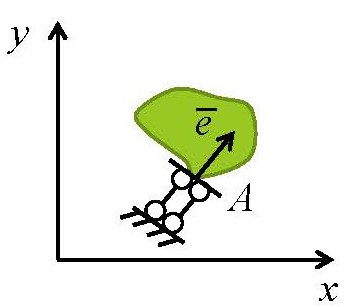
\includegraphics[width=0.15\linewidth]{immagini/1.PARTE3_Pagina_11 (2)}
\end{figure}
MC=2: due informazioni identificano un candidato CdS.

Ricorda che il doppio pendolo impedisce le rotazioni, quindi premettendo le traslazioni il punto sarà improprio. 

\item \textbf{Doppio Doppio Pendolo} $\vec{\Phi} = 0 \Rightarrow ~ \text{se} ~ \exists ~ C \Rightarrow C \rightarrow \infty$
\begin{figure}[H]
	\centering
	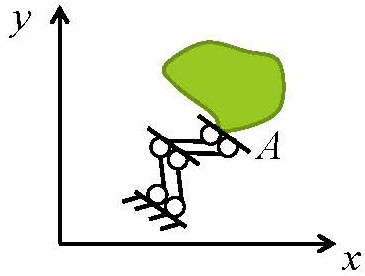
\includegraphics[width=0.15\linewidth]{immagini/1.PARTE3_Pagina_11 (3)}
\end{figure}
\item \textbf{Incastro} $\vec{s_P} = 0 \Rightarrow ~ \forall ~ P \text{ottengo spostamenti banali}  \Rightarrow ~ \nexists C $
\begin{figure}[H]
	\centering
	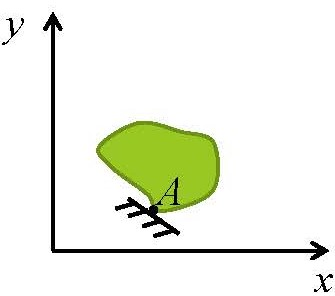
\includegraphics[width=0.15\linewidth]{immagini/1.PARTE3_Pagina_11}
\end{figure}
\item \textbf{Cerniera Interna} $\vec{s_A}^{'', '} = 0 \Rightarrow ~ \text{se} ~ \exists ~ C_{12} \Rightarrow C_{12} \equiv A$
\begin{figure}[H]
	\centering
	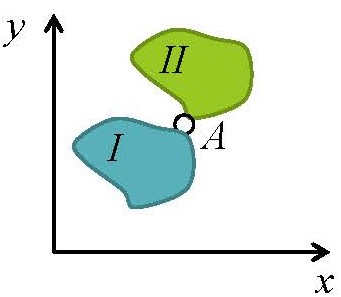
\includegraphics[width=0.15\linewidth]{immagini/1.PARTE3_Pagina_12 (2)}
\end{figure}
\item \textbf{Pendolo Interno} $\vec{s_A}^{'', '} \cdot \vec{e} = 0 \Rightarrow ~ \text{se} ~ \exists ~ C_{12} \Rightarrow C_{12} ~ \in e$
\begin{figure}[H]
	\centering
	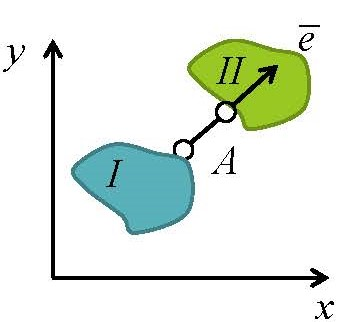
\includegraphics[width=0.15\linewidth]{immagini/1.PARTE3_Pagina_12 (3)}
\end{figure}
\item \textbf{Doppio Pendolo Interno} \newline
$\begin{cases}
	\vec{s_A}^{'', '} \cdot \vec{e} = 0 \\
	\vec{\Phi}^{'', '} = 0
\end{cases} \Rightarrow \begin{cases}
	\text{se} ~ \exists ~ C_{12} \Rightarrow C_{12} ~ \in e\\
	\text{se} ~ \exists ~ C_{12} \Rightarrow C_{12} \rightarrow \infty
\end{cases} \Rightarrow C_{12} \rightarrow \infty ~ \in ~ e$
\begin{figure}[H]
	\centering
	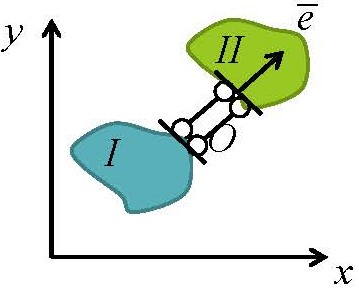
\includegraphics[width=0.15\linewidth]{immagini/1.PARTE3_Pagina_12}
\end{figure}
\item \textbf{Doppio Doppio Pendolo Interno} $\vec{\Phi}^{'', '} = 0 \Rightarrow ~ \text{se} ~ \exists ~ C_{12} \Rightarrow C_{12} \rightarrow \infty$
\begin{figure}[H]
	\centering
	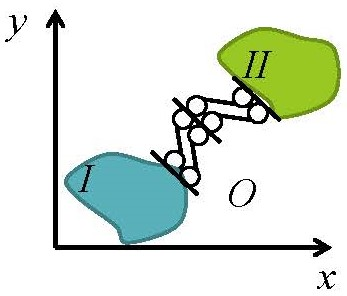
\includegraphics[width=0.15\linewidth]{immagini/1.PARTE3_Pagina_13}
\end{figure}
\end{itemize}

Osservazione: per determinare la posizione di un punto nel piano si necessita di due coordinate, di conseguenza solo i vincoli doppi sono in grado di posizionare il centro di spostamento, mentre quelli singoli lasciano un grado di incertezza. \newline

\newpage

{\Large \textbf{Centro di Spostamento e Labilità}} \mbox{} \newline
L'esistenza del centro fornisce per definizione informazioni sulla possibilità di spostamento: se sono in grado di definire le posizioni del CdS allora il corpo si muove e la labilità sarà non nulla $l\ne0$, valendo il viceversa. \newline
 

Struttura appoggio-appoggio \newline
\begin{figure}[H]
	\centering
	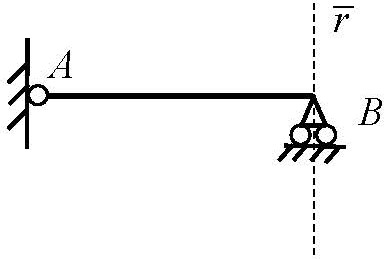
\includegraphics[width=0.15\linewidth]{immagini/1.PARTE3_Pagina_14 (2)}
\end{figure}
\[
\begin{cases}
	A \rightarrow \text{cerniera} \Rightarrow ~ \text{se} ~ \exists ~ C \Rightarrow C \equiv A  \\
	B \rightarrow \text{pendolo o carrello} \Rightarrow ~ \text{se} ~ \exists ~ C \Rightarrow C ~ \in r  
\end{cases}
\]

Il teorema dell'allineamento dice che C dovrebbe essere contemporaneamente sia in A che su r, ovvero allineati: assurdo. Si perviene al fatto che il corpo è fermo e la labilità è perciò nulla: $l=0$. \newline

Rimozione del carrello \newline
\begin{figure}[H]
	\centering
	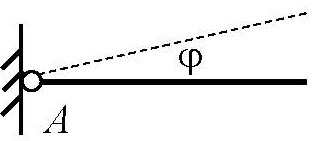
\includegraphics[width=0.15\linewidth]{immagini/1.PARTE3_Pagina_14 (3)}
\end{figure}
\[
	A \rightarrow \text{cerniera} \Rightarrow ~ \text{se} ~ \exists ~ C \Rightarrow C \equiv A
\]
La MC della struttura diviene così pari a 2, le due informazioni contenute nella cerniera mi identificano univocamente il centro di spostamento. 

La cerniera presente blocca due spostamenti possibili: $\rightarrow \uparrow$ l'unico spostamento possibile è la rotazione intorno alla cerniera.

Con un solo spostamento possibile la labilità diviene $l=1$. \newline

Sostituzione della cerniera col carrello \newline
Con questa sostituzione rimuovo il vincolo orizzontale della cerniera. 
\begin{figure}[H]
	\centering
	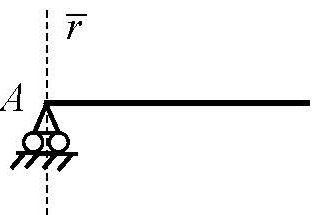
\includegraphics[width=0.15\linewidth]{immagini/1.PARTE3_Pagina_14}
\end{figure}
\[
A \rightarrow \text{pendolo o carrello} \Rightarrow ~ \text{se} ~ \exists ~ C \Rightarrow C ~ \in r 
\]
La MC della struttura si abbassa ad 1, conosco la direzione del candidato CdS, ma non la posizione.

Il pendolo impedisce soltanto gli spostamenti paralleli alla sua direzione $\vec{r}$, il che significa che sono possibili 2 dei 3 spostamenti previsti. 

In particolare $C ~ \in r $ ma si necessita di ancora un'altra coordinata per \underline{fissare} C nel piano, si dice quindi che C ha 1 grado di incertezza: ho la necessità di introdurre un'informazione. \newline 

Quindi, in generale, se $l \ne 0$ e cioè se $\exists ~ C$, la labilità è nota attraverso:
\[
l = 1 + g
\]
Dove $g$ è il numero di informazioni arbitrarie che è necessario introdurre per trovare univocamente, senza incertezze, C. \newline


\textbf{Serie di esempi} \newline

\begin{enumerate}

\item \mbox{}

\begin{figure}[H]
	\centering
	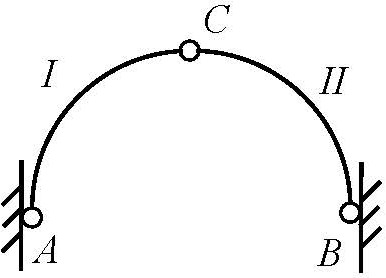
\includegraphics[width=0.15\linewidth]{immagini/1.PARTE3_Pagina_15 (2)}
\end{figure}
\[
A \rightarrow \text{cerniera} \Rightarrow ~ \text{se} ~ \exists ~ C_1 \Rightarrow C_1 \equiv A
\]
\[
B \rightarrow \text{cerniera} \Rightarrow ~ \text{se} ~ \exists ~ C_2 \Rightarrow C_2 \equiv B
\]
\[
C \rightarrow \text{cerniera} \Rightarrow ~ \text{se} ~ \exists ~ C_{12} \Rightarrow C_12 \equiv C
\]
Ma $C_1, C_2, C_{12}$ non sono e non possono essere allineati, non esiste una retta che li contenga tutte e tre, perciò l'unico spostamento possibile sarà quello banale, nullo, il corpo è fermo $l=0$ \newline

\item \mbox{}

\begin{figure}[H]
	\centering
	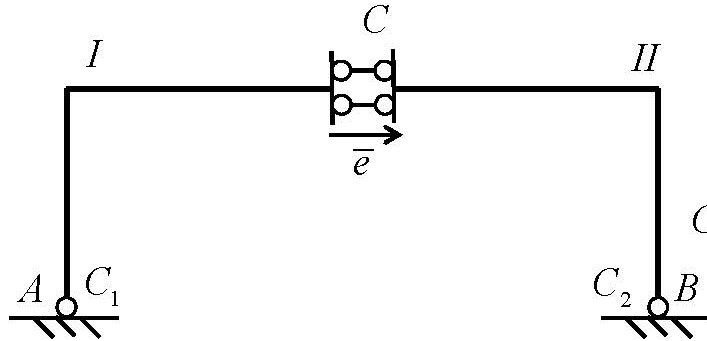
\includegraphics[width=0.25\linewidth]{immagini/1.PARTE3_Pagina_15}
\end{figure}
\[
A \rightarrow \text{cerniera} \Rightarrow ~ \text{se} ~ \exists ~ C_1 \Rightarrow C_1 \equiv A
\]
\[
B \rightarrow \text{cerniera} \Rightarrow ~ \text{se} ~ \exists ~ C_2 \Rightarrow C_2 \equiv B
\]
\[
C \rightarrow \text{doppio pendolo} \Rightarrow ~ \text{se} ~ \exists ~ C_{12} \Rightarrow C_12 \rightarrow \infty ~ \in \vec{e}
\]
Poiché  $C_{12}$ è all'infinito non c'è modo di non credere che $C_{12}$ all'infinito sia allineato a $C_1, C_2$, e i tre punti si possono considerare allineati. 

Se inoltre $C_{12}$ appartiene alla retta per $\overline{AB}$, risulta spazialmente fissato e quindi $g=0$;
\[
l = 1+ g = 1
\] 
2 punti proprio ed uno improprio sono allineati se i due punti propri giacciono su una retta parallela a quella che identifica la direzione di un punto improprio.  

\newpage


\item \mbox{}
\begin{figure}[H]
	\centering
	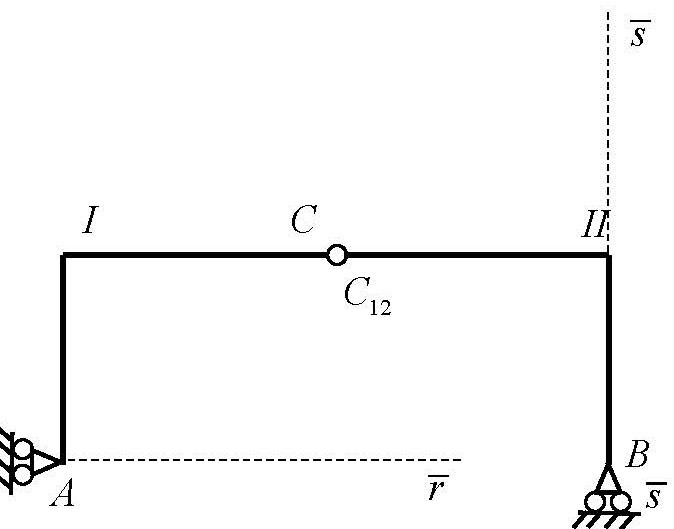
\includegraphics[width=0.25\linewidth]{immagini/1.PARTE3_Pagina_16 (2)}
\end{figure}
\[s=4; t = 2\]
Ho bisogno di tre centri e dunque  informazioni per trovarli tutti univocamente.
\[
A \rightarrow \text{carrello} \Rightarrow C_1 ~ \in  \vec{r}
\]
\[
B \rightarrow \text{carrello} \Rightarrow C_2 ~ \in  \vec{s}
\]
\[
C \rightarrow \text{cerniera} \Rightarrow C_12 \equiv C
\]
Si può tracciare una qualsiasi retta che dimostri come $C_1, C_2, C_{12}$ siano allineati, con la condizione per cui $C_1, C_2$ sono da scegliersi in maniera arbitraria, a partire da $C_{12}$ che fornisce la posizione di $C_1$ sulla retta $\vec{r}$ e in seguito quella di $C_2$ sulla retta $\vec{s}$.

Ci si accorge in questo modo che si è dovuto scegliere un parametro e dunque $g = 1 \Rightarrow l = 1+g = 2$: per poter fissare i centri di spostamento, è necessario fissare arbitrariamente o $C_1$ o $C_2$. 

\newpage

\item \mbox{}

\begin{figure}[H]
	\centering
	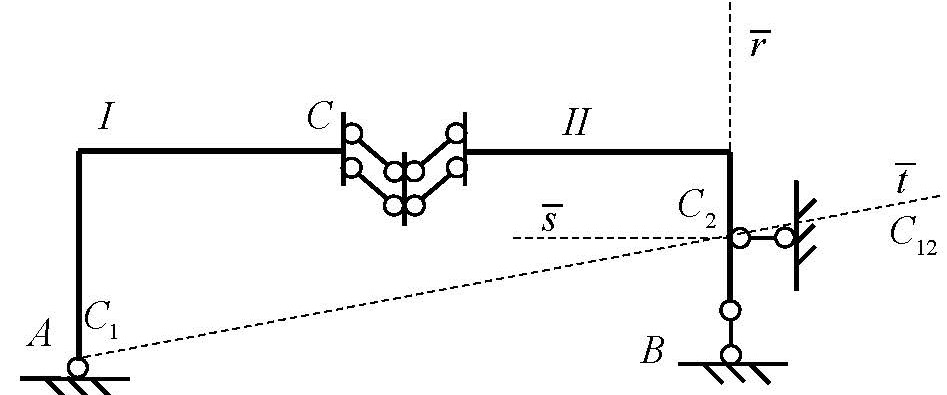
\includegraphics[width=0.4\linewidth]{immagini/1.PARTE3_Pagina_16}
\end{figure}
\[s = 5; t = 2 \Rightarrow 6 ~ \text{informazioni necessarie}\]
Corpo 1 vincoli esterni: Cerniera A $C_1 \equiv A$ \newline

Corpo 2 vincoli esterni: Pendolo B $C_2 \in \vec{r}$, Pendolo D $C_2 \in \vec{s}$ e dunque $C_2 = \left\lbrace \vec{r} \bigcap \vec{s}\right\rbrace$ \newline

Vincoli interni: Doppio Doppio Pendolo C $C_{12} \rightarrow \infty$ \newline

Perciò con $C_1 \equiv A$, $C_2 = \left\lbrace \vec{r} \bigcap \vec{s}\right\rbrace$, $C_{12} \rightarrow \infty$ i tre punti sono allineati se e solo se sono allineati $C_1, C_2$.

$C_1, C_2$ sono allineati sulla retta $\vec{t}$ e questi significa che $C_{12}$ apparterrà all'infinito a tale retta e non diviene più necessario scegliere nemmeno un parametro per identificare i centri di spostamento $g=0 \Rightarrow l = 1+g = 1$: $C_{12}$ è univocamente determinato dagli univocamente determinati $C_1, C_2$. 

\item \mbox{}

\begin{figure}[H]
	\centering
	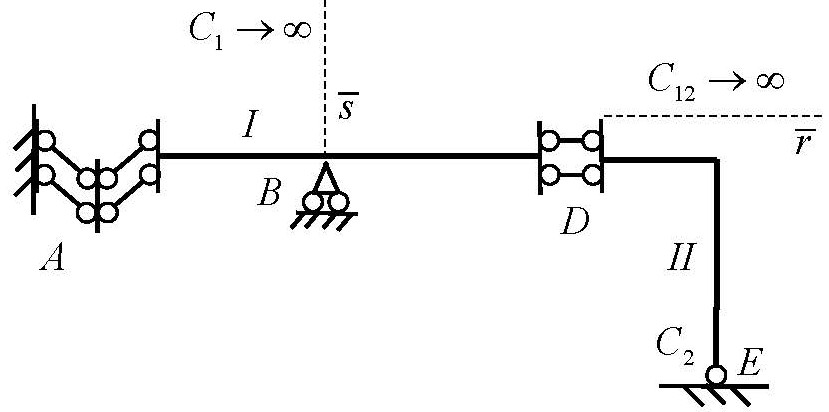
\includegraphics[width=0.4\linewidth]{immagini/1.PARTE3_Pagina_17 (2)}
\end{figure}
Corpo 1 vincoli esterni: Doppio Doppio Pendolo A $C_{1} \rightarrow \infty$, Pendolo B $C_1 \in \vec{s}$ allora $C_1 \rightarrow \infty ~ \in \vec{s}$ \newline

Corpo 2 vincoli esterni: Cerniera E $C_2 \equiv E$ \newline

Vincoli interni: Doppio Pendolo D $C_{12} \rightarrow \infty ~ \in \vec{r}$\newline

Poiché $C_{1}$ è all'infinito lungo $\vec{s}$, $C_{12}$ è all'infinito lungo $\vec{r}$ e $C_2 \equiv E$, non c'è alcuna possibilità che $C_1, C_2, C_{12}$ siano allineati e perciò $l = 0$. 
$C_{1}$ e $C_{12}$ sono all'infinito lungo direzioni diverse. \newline

Due punti impropri ed uno proprio, sono allineati se e solo se le direzioni dei due punti impropri sono parallele. \newline
\newpage
\item \mbox{}

\begin{figure}[H]
	\centering
	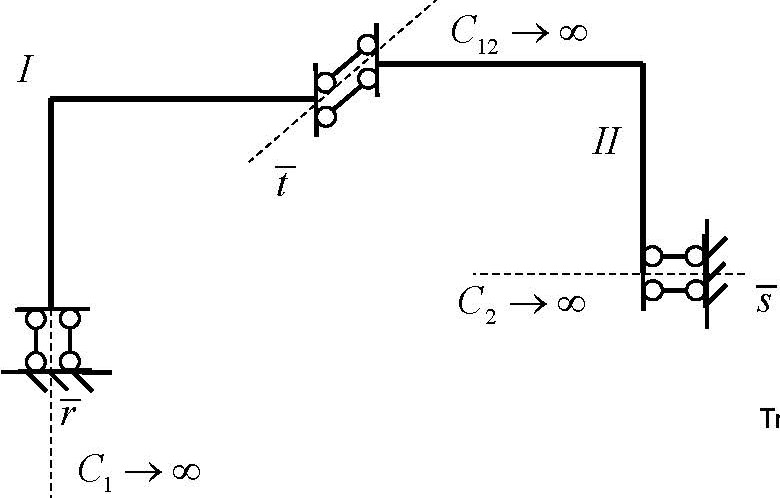
\includegraphics[width=0.4\linewidth]{immagini/1.PARTE3_Pagina_17}
\end{figure}
Corpo 1 vincoli esterni: Doppio Pendolo A $C_{1} \rightarrow \infty ~ \in \vec{r}$ \newline

Corpo 2 vincoli esterni: Doppio Pendolo A $C_{2} \rightarrow \infty ~ \in \vec{s}$ \newline

Vincoli interni: Doppio Pendolo C $C_{12} \rightarrow \infty ~ \in \vec{t}$\newline

$C_1, C_2, C_{12}$ sono all'infinito lungo tre direzioni diverse, essi sono allineati e univocamente definiti: $g=0 \Rightarrow l=1$ \newline

Tre punti impropri sono sempre allineati. \newline

\end{enumerate}

{\Large \textbf{Centro di Spostamento e Catene Cinematiche}} \mbox{} \newline

Conoscendo i centri di spostamento si possono facilmente e \underline{qualitativamente} tracciare le catene cinematiche, tracciando gli spostamenti come rotazioni intorno ai centri di spostamento. \newline

\textbf{Esempio 1} \newline
Esempio già visto l=1, ho un parametro libero, decido di fissare arbitrariamente la rotazione.

Con $l = 1+n$ si dovranno fissare n parametri più quello che si andrà a tracciare.
\begin{figure}[H]
	\centering
	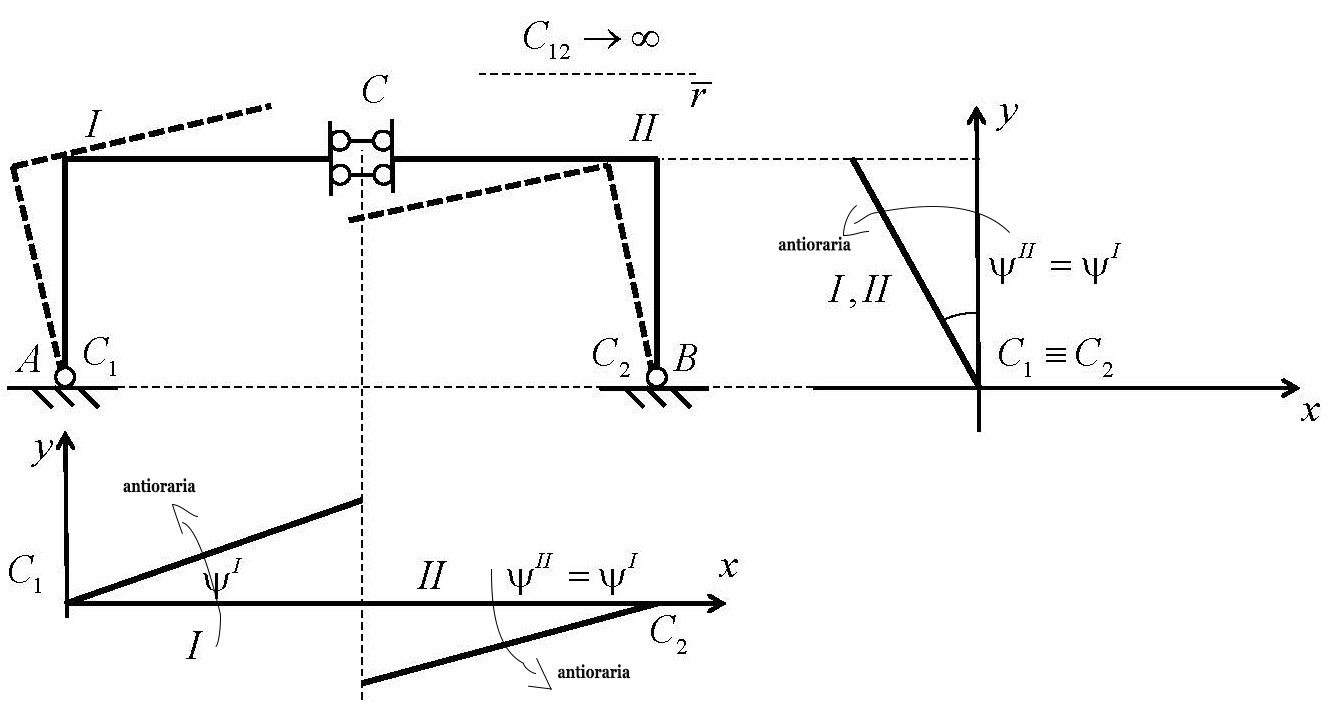
\includegraphics[width=0.65\linewidth]{immagini/1.PARTE3_Pagina_18}
\end{figure}
\begin{enumerate}
\item Individuare i centri di spostamento \newline
Cerniera A $C_1 \equiv A$ \newline
Cerniera B $C_2 \equiv B$ \newline
Doppio Pendolo C $C_{12} \rightarrow \infty ~ \in \vec{t}$\newline

$C_1, C_2, C_{12}$ allineati $\Rightarrow g = 0 \Rightarrow l = 1$ \newline 

Le rotazioni in un grafico di spostamenti corrispondono parametricamente alla pendenza di un grafico a rotazione costante: pendenza costante $\Rightarrow$ retta/segmento rettilineo.

\item Rappresentare gli spostamenti come rotazioni pure intorno al centro di spostamento, unico punto che non si muove. 

$l =1$ dunque si può scegliere arbitrariamente un solo parametro, solitamente l'angolo di spostamento.

Corpo 1: spostamento su $ y $ di $\varphi'$. \newline
Corpo 2: spostamento su $ y $ di $\varphi'' = \varphi'$ parallelo a quello del corpo 1 a causa del doppio pendolo interno. \newline
Corpo 1 e Corpo 2: spostamenti su $ x $ perpendicolari a quelli su $ y $. \newline

Il doppio pendolo dice inoltre che la rotazione relativa è nulla e dunque le rotazioni tra i due corpo sono uguali: stessa rotazione = stessa pendenza $\Rightarrow$ diagramma parallelo a quello del primo corpo. 
\end{enumerate}

\textbf{Esempio 2} \newline
\begin{figure}[H]
	\centering
	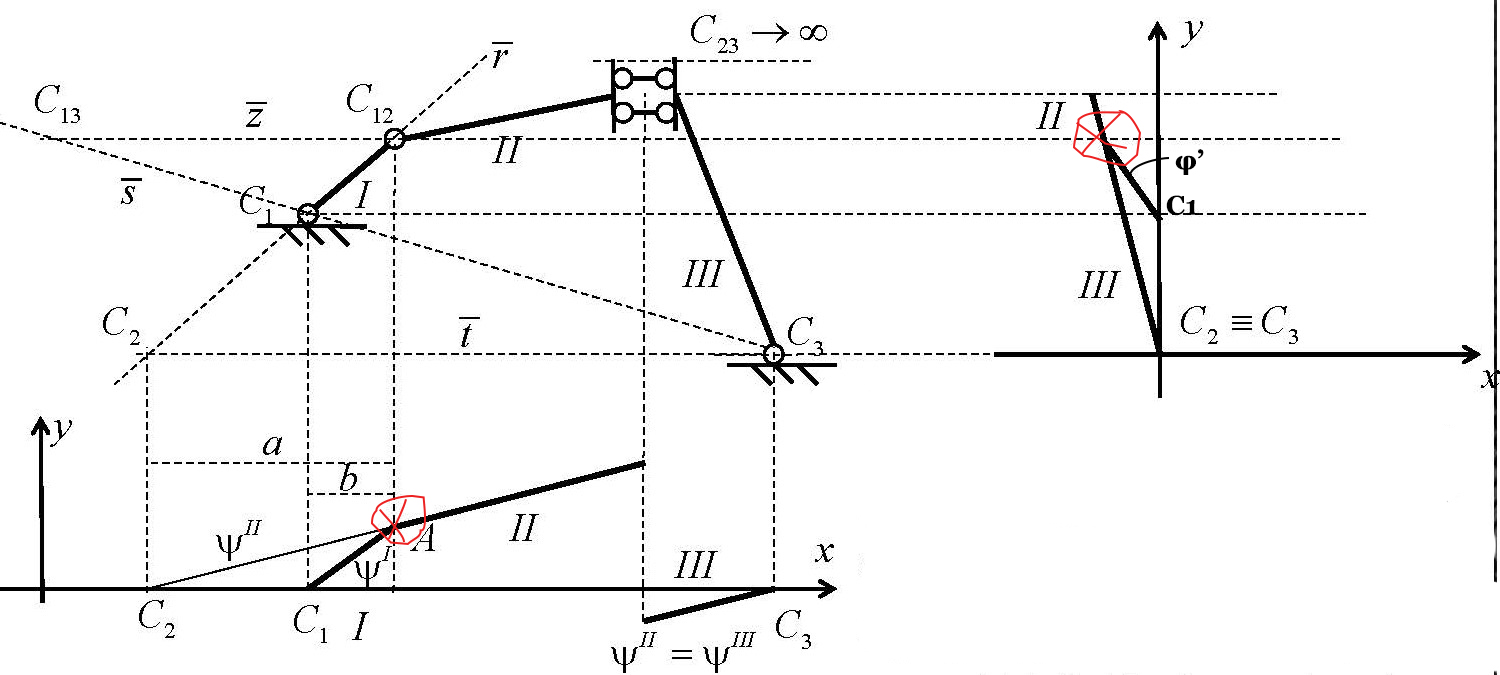
\includegraphics[width=0.65\linewidth]{immagini/1.PARTE3_Pagina_20}
\end{figure}


\[ s=8; t=3 \Rightarrow CdS = 6 \Rightarrow 12 ~ info\]

\begin{enumerate}
	\item Vincoli esterni 
	\begin{itemize}
		\item[I] $C_1$ è univocamente determinato;
		\item[II] $C_2$ si trova dal fatto che deve essere allineato a $C_1$ e $C_{12}$, da questi so che apparterrà alla retta $r$;
		\item[III] $C_3$ è univocamente determinato;
	\end{itemize}

	\item Vincoli interni
	\begin{itemize}
		\item[I-II]  $C_{12}$ è univocamente determinato;
		\item[II-III] $C_{23} \rightarrow \infty \in ~  e$;
	 	\item[I-III] $C_{13}$ è noto dal fatto che dev'essere allineato a $C_1$ e $C_3$, e dunque deve appartenere alla retta $s$.
	\end{itemize}
	\item Allineamento
	\begin{itemize}
		\item $C_1, C_2, C_{12}$ allineati;
		\item $C_2, C_{23}, C_3$ allineati solo se appartenenti alla retta $t$, $C_{23}$ è improprio lungo la retta $t \parallel e$: allineati;
		\item $C_1, C_{13}, C_3$ allineati lungo la retta s;
		\item $C_{12}, C_{13}, C_{23}$ allineati solo se appartengono alla retta $z$, $C_{23}$ è improprio lungo la retta $t \parallel z$: allineati;
	\end{itemize}	
\end{enumerate}

Ho univocamente determinato tutti i CdS $\Rightarrow g=0 \Rightarrow l=1$ \newline 

Spostamenti lungo y: 
\begin{itemize}
	\item Corpo I: rotazione intorno a $C_1$ arbitraria dell'angolo $\varphi_1$.
	\item Corpo II: Rotazione intorno a $C_2$. La cerniera interna $C_{12}$ dà l'informazione che le rotazioni sono libere mentre impone spostamenti relativi nulli $\begin{cases}
		s'_{Bx} = s''_{Bx} \\
		s'_{By} = s''_{By} 
	\end{cases}$, il punto \textcolor{red}{$\textbf{X}$} in figura è tale per cui $s'_{By} = s''_{By}$, siccome so che il corpo II comincia appena finisce il corpo I, e con la conoscenza dell'ubicazione di $C_2$, la retta descrivente lo spostamento del corpo II sarà perciò quella passante per $C_2$ ed \textcolor{red}{$\textbf{X}$}.

	 L'inclinazione è possibile calcolarla conoscendo che: 
\[ \varphi_1 \cdot b = \varphi_2 \cdot a \]
	\item Corpo III: il doppio pendolo interno da informazioni sul fatto che le rotazioni sono identiche, la retta descrivente allora lo spostamento avrà la stessa pendenza e sarà parallela a quella del corpo II, passante per $C_3$: 
	\[\varphi_3 = \varphi_2\]
\end{itemize}

Spostamenti lungo x: \newline 
È noto per definizione che $C_1 \equiv C_3$ e $C_1$ hanno spostamento nullo lungo $x$ e che $C_{12}$ impone lo stesso spostamento relativo $s'_{Bx} = s''_{Bx}$. 

Si cominci dal corpo I, avrà lo stesso spostamento imposto arbitrariamente prima ovvero $\varphi_1$, dal corpo I parte il corpo II non appena arriva ad \textcolor{red}{$\textbf{X}$}, e il corpo III ha la stessa pendenza del corpo III. 

Un ulteriore controllo può essere fornito dal fatto che gli spostamenti sui rispettivi grafici devono essere tra loro ortogonali. \newline 

\textbf{Esempio 3} \newline
\begin{figure}[H]
	\centering
	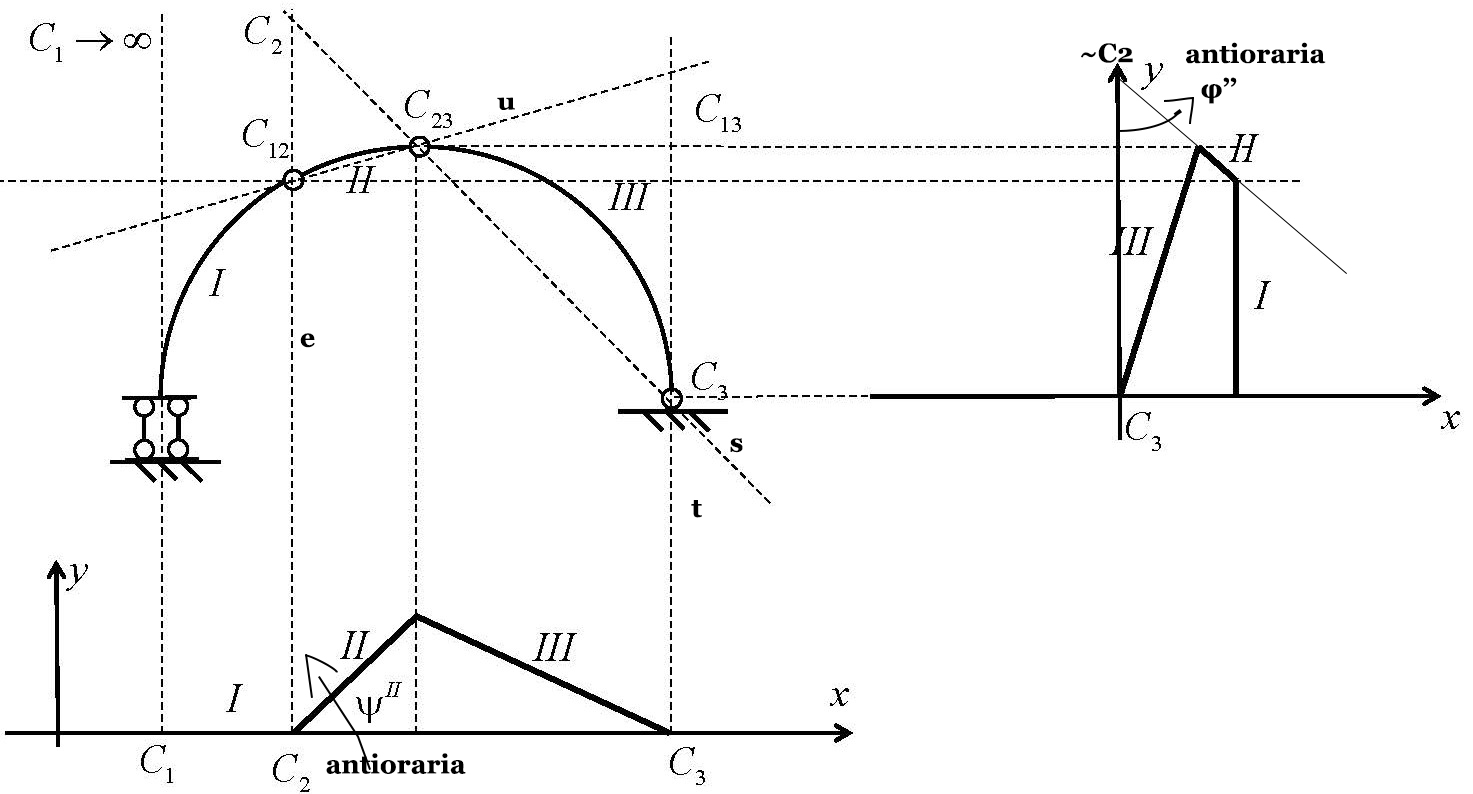
\includegraphics[width=0.65\linewidth]{immagini/1.PARTE3_Pagina_21}
\end{figure}
\[ s=8; t=3 \Rightarrow CdS = 6 \Rightarrow 12 ~ info\]
\begin{enumerate}
	\item Vincoli esterni 
	\begin{itemize}
		\item[I] $C_1 \rightarrow \infty \in ~  e$;
		\item[II] $C_2$ si trova dal fatto che deve essere allineato a $C_1$, ovvero parallelo alla sua direzione, e a $C_{12}$, quindi apparterrà alla retta $e$, inoltre $C_2, C_{23}, C_3$ devono essere allineati e lo sono soltanto se appartengono alla retta $s$;
		\item[III] $C_3$ è univocamente determinato;
	\end{itemize}
	
	\item Vincoli interni
	\begin{itemize}
		\item[I-II]  $C_{12}$ è univocamente determinato;
		\item[II-III] $C_{23}$ è univocamente determinato;
		\item[I-III] $C_{13}$ è noto dal fatto che dev'essere allineato a $C_1$ e $C_3$, e lo è solo se $t\parallel e$, inoltre $C_{12}, C_{23}, C_{13}$ sono allineati solo se appartengono alla retta $u$.
	\end{itemize}
	\item Allineamento
	\begin{itemize}
		\item $C_1, C_2, C_{12}$ allineati se $C_2 \in r \parallel e$;
		\item $C_2, C_{23}, C_3$ allineati se $C_3 \in s$;
		\item $C_1, C_{13}, C_3$ se $C_{13} \in t \parallel e$;;
		\item $C_{12}, C_{13}, C_{23}$ allineati solo se $C_{13} \in u$
	\end{itemize}	
\end{enumerate}
Ho univocamente determinato tutti i CdS $\Rightarrow g=0 \Rightarrow l=1$ \newline

Spostamenti lungo y: 
\begin{itemize}
	\item Corpo I: nulli. 
	
	Il corpo I non si muove in direzione y, vincolato esternamente con un doppio pendolo, esso può traslare ma non può ruotare. In che modo trasla? Per definizione le traslazioni sono perpendicolari al centro di spostamento, in questo caso a $C_1$, essendo così il centro posto all'infinito lungo la verticale, la traslazione sarà orizzontale. 
	\item Corpo II: è possibile così per questo corpo assegnare un parametro libero, che sia $\varphi_2$ in senso antiorario rispettando lo spostamento nullo di $C_2$ in $y$ con l'inizio e la fine dei rispettivi corpi (dove finisce uno parte l'altro). 
	\item Corpo III: il diagramma dello spostamento del corpo III soddisfa il fatto che a quota $C_3$ lo spostamento è nullo, mentre a $C_{23}$ varrà $s''_y = s'''_y$ con una retta individuata per due punti. 
\end{itemize} 

Spostamenti lungo x: \newline
Si comincia a tracciare il grafico dal primo valore noto: $\varphi_2$ antiorario con la nota posizione di $C_2$ a spostamento nullo, tracciato nel campo di definizione del corpo II, nota la posizione di $C_3$ si traccia lo spostamento tra inizio e fine del corpo rispettando che in $C_{23} ~ s''_x = s'''_x$, si traccerà infine lo spostamento del corpo I, nel suo campo d'appartenenza, valendo in $C_{123} ~ s'_x = s''_x$, con spostamenti ortogonali tra i due rispettivi grafici. 

\newpage
{\Large \textbf{NOTE}}





	
	%	\vfill
%\begin{tcolorbox}[height=4.5cm]
%	This box has a height of 1cm.
%\end{tcolorbox}
		
	\end{adjustwidth}
\end{document}